\begin{figure}[h]
    \centering
    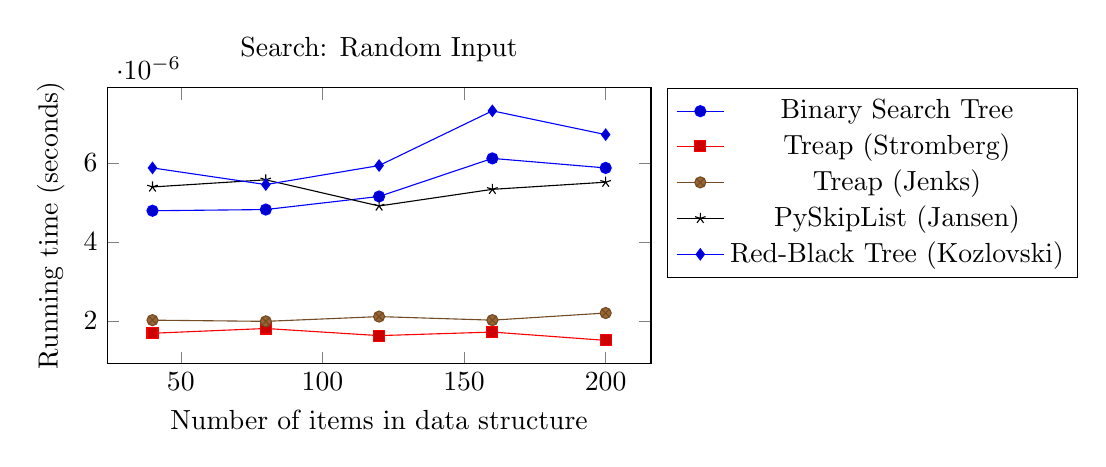
\begin{tikzpicture}
        \begin{axis}[
            xlabel={Number of items in data structure},
            ylabel={Running time (seconds)},
            title={Search: Random Input},
            width=0.7\textwidth,
            height=2in,
            legend pos=outer north east
        ]
		\addplot coordinates {
			(40, 4.78868785435127e-06)
			(80, 4.818805388029368e-06)
			(120, 5.1500982584523625e-06)
			(160, 6.113859336059901e-06)
			(200, 5.872919066657323e-06)
		};
		\addplot coordinates {
			(40, 1.686581885806948e-06)
			(80, 1.807052020511013e-06)
			(120, 1.626346818459079e-06)
			(160, 1.716699419485046e-06)
			(200, 1.5058766837577896e-06)
		};
		\addplot coordinates {
			(40, 2.017874756235494e-06)
			(80, 1.987757222562947e-06)
			(120, 2.108227357261461e-06)
			(160, 2.017874756235494e-06)
			(200, 2.198579958287428e-06)
		};
		\addplot coordinates {
			(40, 5.391038527854941e-06)
			(80, 5.571743729906875e-06)
			(120, 4.9091579890525596e-06)
			(160, 5.3308034605042964e-06)
			(200, 5.511508662553455e-06)
		};
		\addplot coordinates {
			(40, 5.872919066657323e-06)
			(80, 5.451273595205586e-06)
			(120, 5.933154134007967e-06)
			(160, 7.318560683064468e-06)
			(200, 6.716210009560797e-06)
		};
        \legend{Binary Search Tree, Treap (Stromberg), Treap (Jenks), PySkipList (Jansen), Red-Black Tree (Kozlovski)}
        \end{axis}
    \end{tikzpicture}
    \caption{Average of 10 operations, benchmarked every 40, starting at 40.}
\end{figure}